\documentclass[10pt,a4paper]{article}
\usepackage[utf8]{inputenc}
\usepackage{amsfonts}
\usepackage{graphicx}
\usepackage[letterpaper, margin=1in]{geometry}
\usepackage{indentfirst}
\usepackage{tikz,pgfplots}
\usepackage{float}

\begin{document}

\title{Final: Deep NLP}
\author{Alex Shah}
\date{12/7/17}

\maketitle

\section{Strategy}

My strategy to determine which parameters to change was to research and recall the effects of each parameter on the data. For example I knew batch size would have little effect on the end results but may speed up the processing of the dataset, depending on the hardware. Since time was not of the essence to train a few epochs, I decided to focus my attention on other parameters. In this model, the only parameters which have an affect other than epochs, are the hidden units, number of recurrent steps, number of layers, and keep probability.

\section{Most Influential Parameters}

I knew right away that some of the most influential parameters would be the number of hidden units and number of layers. Increasing these parameters would increase the overall computation space therefore increasing training time, but would most likely improve perplexity (ie decrease the value). I did not expect the best results to be from increasing the number of steps to 50. In retrospect it does make sense that increasing the number of recurrence steps would improve results. By combining the three most influential parameters the results improved even more dramatically. I also did not expect that the number of layers made nearly no difference to the training, validation, and test perplexities. The only change made by increasing the number of layers was lowering the initial perplexity which quickly fell into step with the default run.

\section{Least Influential Parameters}

Most likely this code was not optimized for changing the dropout layer. It was intially set to 1 and the results of decreasing the keep probability were adverse at worst and roughly the same at best. It would not effect results to change some of the other paramaters, other than causing vanishing/exploding gradient or other related problems. Initial weight scale would not change the results. IIncreasing the initial learning rate would make results worse until the learning rate begins to drop, and starting low would adversely affect the model. The max gradient norm just prevents against exploding gradient. Epoch related parameters involve the number of epochs at the initial training rate, then the amount of training epochs. As with any mode, more epochs would approach a better perplexity at the cost of time. Batch size, vocab size, etc, are related to processing the data and would not affect results. So the least influential of the parameters which affect perplexity was keep probability, which was only 2.



\begin{figure}[t]
  \begin{center}
    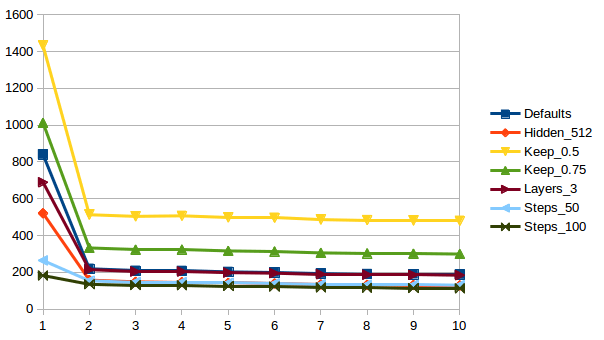
\includegraphics[width=0.75\textwidth]{epochs1.png}
    \caption{Test parameters over third epoch}
  \end{center}
\end{figure}


\begin{figure}[b]
  \begin{center}
    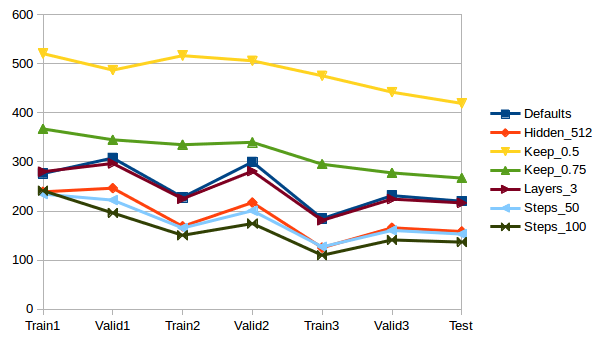
\includegraphics[width=0.75\textwidth] {train-valid-test1.png}
    \caption{Training, Validation, and Test Perplexity}
  \end{center}
\end{figure}

\clearpage

\section{Best Runs Combined}

Combining the three best attributes proved to have excellent results. The changes made to the default hyperparameters were:

Number of Layers: 3

Number of Steps: 100

Hidden Size: 512

\begin{figure}[H]
  \begin{center}
    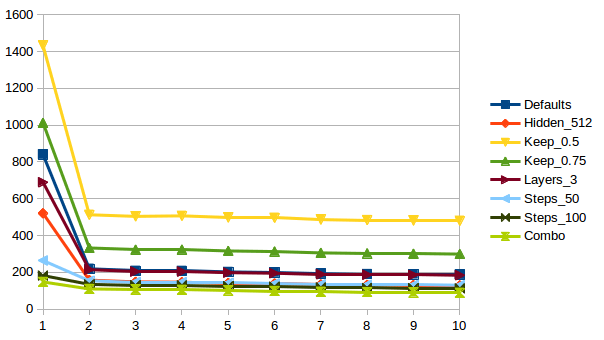
\includegraphics[width=0.75\textwidth] {epochs2.png}
    \caption{Combining Best hyperparameter changes}
  \end{center}
\end{figure}

\begin{figure}[H]
  \begin{center}
    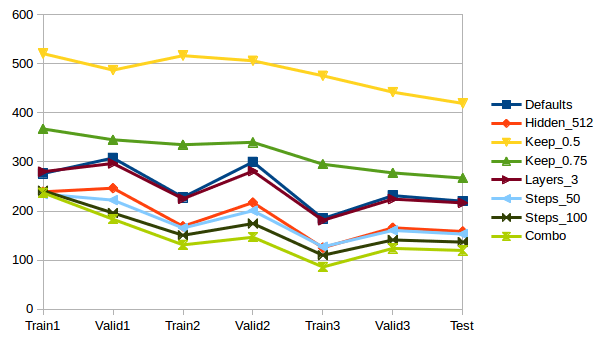
\includegraphics[width=0.75\textwidth] {train-valid-test2.png}
    \caption{Combining Best hyperparameter changes}
  \end{center}
\end{figure}

\clearpage

\section{Sentences}

\subsection{}

The default hyperparameters produced the following output:

Epoch 1: the company will be used in a [unk] test in a [unk] test in a [unk] test in a [unk] test

Epoch 2: the company said eos unk said it will be used in a [unk] test in a [unk] test in a [unk]

Epoch 3: the company said [eos] [unk] said it will be a [unk] in a [unk] [unk] in a [unk] [unk] in a

Test Perplexity: 220.851

-----

The sentences the default hyperparameters generated seemed to get stuck in a loop. Maybe from the limited number of epochs it was unable to capture significant information to make 20 words worth of text. The initial 3 to 5 words were more sentence-like, but quickly reverted to repetition.

\subsection{}

The combination of best factors produced the following sentences:

Epoch 1: the fed 's largest trade deficit [eos] the [unk] of the [unk] of the [unk] of the [unk] of the [unk]

Epoch 2: the largest trade index is n't expected to be in the u.s. market [eos] the fed has n't been able to

Epoch 3: the largest largest west german national league of the u.s. intelligence committee [eos] the fed has been [unk] with the u.s.

-----

The combination of factors which produced the lowest perplexity also produced the most comprehensible sentences. The first sentence had repitiion like the default hyperparameters runs, however by the second and third epochs the sentences contained longer strings of words which made logically sense.

\section{Mark/Trump Datasets}

\subsection{Mark Results}
Combo hyperparameters:


- Number of layers: 3


- Hidden units: 512


- Recurrent steps: 100


Running the default and combo hyperparameters gave the following results:



\begin{figure}[H]
  \begin{center}
    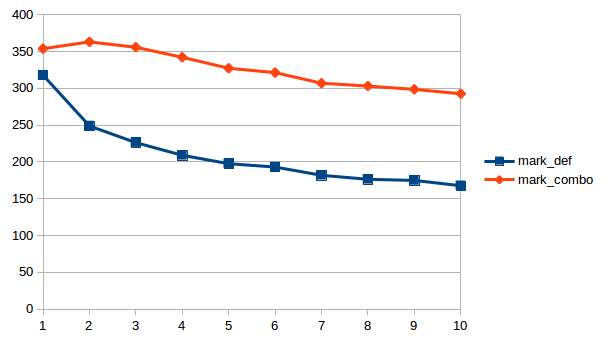
\includegraphics[width=0.75\textwidth] {mark1.png}
    \caption{Default and Combo hyperparameters on Mark Dataset; third epoch}
  \end{center}
\end{figure}

\begin{figure}[H]
  \begin{center}
    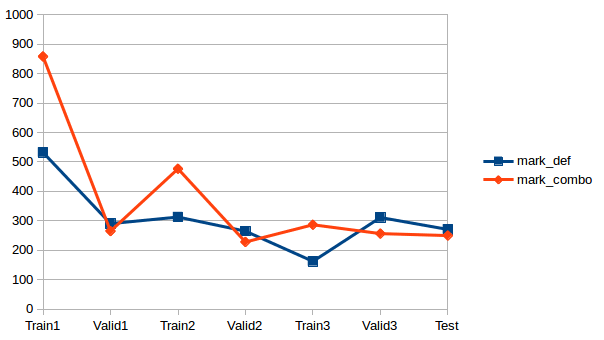
\includegraphics[width=0.75\textwidth] {mark2.png}
    \caption{Default and Combo hyperparameters on Mark Dataset; training, validation, and test}
  \end{center}
\end{figure}

We can see from the perplexity results in figures 5 and 6 that the combo hyperparameters proved effective in decreasing perplexity, though not by as much as the PTB dataset.

\subsection{Mark Sentences}
Default:


Epoch 1: the Lord had right the Lord will the Lord the Lord had right the Lord will the Lord the Lord had

Epoch 2: the right news the right will be right will be right will be right will be right will be right will

Epoch 3: the news and the Lord who will not been one who will not believe the good news the right news out

The default hyperparameters were able to capture some semblance of sentence structure or at least variation in words output.

-----

Combo:


Epoch 1: the the the the the the the the the the the the the the the the the the the the the

Epoch 2: the the the the the the the the the the the the the the the the the the the the the

Epoch 3: the chief they will not the whole he will be the whole the whole they will not the whole he will

The combo hyperparameters seemed to get stuck more easily, early on. For 2 epochs the strongest association to "the" was "the" leading to an infinite loop. It was able to break out of this by epoch 3.

\subsection{Trump Results}

\begin{figure}[H]
  \begin{center}
    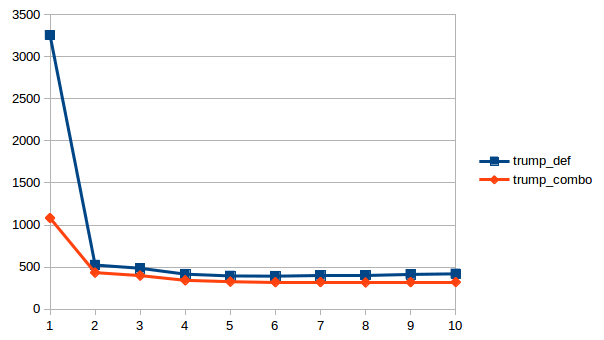
\includegraphics[width=0.75\textwidth] {trump1.png}
    \caption{Default and Combo hyperparameters on Trump Dataset; third epoch}
  \end{center}
\end{figure}

\begin{figure}[H]
  \begin{center}
    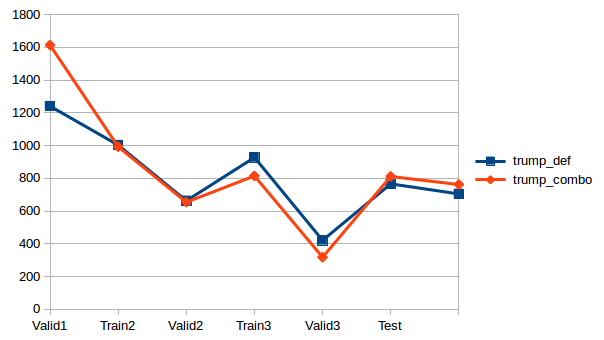
\includegraphics[width=0.75\textwidth] {trump2.png}
    \caption{Default and Combo hyperparameters on Trump Dataset; training, validation, and test}
  \end{center}
\end{figure}

Changing hyperparameters had less of an effect on the Trump dataset. The vocabulary size for this dataset was more than triple the vocabulary size for PTB. This, coupled with complexities related to twitter such as usernames, hashtags, etc, could have led to the results we see with diminished effect of the combo hyperparameters compared to the previous datasets.

\subsection{Trump Sentences}
Default:


Epoch 1: the Obama is a great time of the Obama is a great time of the Obama is a great time of

Epoch 2: the @Yankees thing you can do well in the next debate. -- @MittRomney will be a great time to the debate

Epoch 3: the @Yankees game of the @Yankees game last night. <eos>I have to do well in the debate of the @Yankees game

The sentences generated by the default hyperparameters were repetitive and random. But they still read like proper Trump tweets.



Combo:


Epoch 1: the debate of the debate of the debate of the debate of the debate of the debate of the debate of

Epoch 2: the @Yankees in the world is a total in the debate of the next season of Obama to the debate of

Epoch 3: the most most years of the world in the world is the most important in the world in the debate he

The combo hyperparameters led to more structured sentences but, like in the Mark dataset, was initially more repetitive. 

\end{document}